\documentclass{article}\usepackage[]{graphicx}\usepackage[]{xcolor}
% maxwidth is the original width if it is less than linewidth
% otherwise use linewidth (to make sure the graphics do not exceed the margin)
\makeatletter
\def\maxwidth{ %
  \ifdim\Gin@nat@width>\linewidth
    \linewidth
  \else
    \Gin@nat@width
  \fi
}
\makeatother

\definecolor{fgcolor}{rgb}{0.345, 0.345, 0.345}
\newcommand{\hlnum}[1]{\textcolor[rgb]{0.686,0.059,0.569}{#1}}%
\newcommand{\hlstr}[1]{\textcolor[rgb]{0.192,0.494,0.8}{#1}}%
\newcommand{\hlcom}[1]{\textcolor[rgb]{0.678,0.584,0.686}{\textit{#1}}}%
\newcommand{\hlopt}[1]{\textcolor[rgb]{0,0,0}{#1}}%
\newcommand{\hlstd}[1]{\textcolor[rgb]{0.345,0.345,0.345}{#1}}%
\newcommand{\hlkwa}[1]{\textcolor[rgb]{0.161,0.373,0.58}{\textbf{#1}}}%
\newcommand{\hlkwb}[1]{\textcolor[rgb]{0.69,0.353,0.396}{#1}}%
\newcommand{\hlkwc}[1]{\textcolor[rgb]{0.333,0.667,0.333}{#1}}%
\newcommand{\hlkwd}[1]{\textcolor[rgb]{0.737,0.353,0.396}{\textbf{#1}}}%
\let\hlipl\hlkwb

\usepackage{framed}
\makeatletter
\newenvironment{kframe}{%
 \def\at@end@of@kframe{}%
 \ifinner\ifhmode%
  \def\at@end@of@kframe{\end{minipage}}%
  \begin{minipage}{\columnwidth}%
 \fi\fi%
 \def\FrameCommand##1{\hskip\@totalleftmargin \hskip-\fboxsep
 \colorbox{shadecolor}{##1}\hskip-\fboxsep
     % There is no \\@totalrightmargin, so:
     \hskip-\linewidth \hskip-\@totalleftmargin \hskip\columnwidth}%
 \MakeFramed {\advance\hsize-\width
   \@totalleftmargin\z@ \linewidth\hsize
   \@setminipage}}%
 {\par\unskip\endMakeFramed%
 \at@end@of@kframe}
\makeatother

\definecolor{shadecolor}{rgb}{.97, .97, .97}
\definecolor{messagecolor}{rgb}{0, 0, 0}
\definecolor{warningcolor}{rgb}{1, 0, 1}
\definecolor{errorcolor}{rgb}{1, 0, 0}
\newenvironment{knitrout}{}{} % an empty environment to be redefined in TeX

\usepackage{alltt}
\usepackage[sc]{mathpazo}
\renewcommand{\sfdefault}{lmss}
\renewcommand{\ttdefault}{lmtt}
\usepackage[T1]{fontenc}
\usepackage{geometry}
\geometry{verbose,tmargin=2.5cm,bmargin=2.5cm,lmargin=2.5cm,rmargin=2.5cm}
\setcounter{secnumdepth}{2}
\setcounter{tocdepth}{2}
\usepackage[unicode=true,pdfusetitle,
 bookmarks=true,bookmarksnumbered=true,bookmarksopen=true,bookmarksopenlevel=2,
 breaklinks=false,pdfborder={0 0 1},backref=false,colorlinks=false]
 {hyperref}
\hypersetup{
 pdfstartview={XYZ null null 1}}

\makeatletter
%%%%%%%%%%%%%%%%%%%%%%%%%%%%%% User specified LaTeX commands.
\renewcommand{\textfraction}{0.05}
\renewcommand{\topfraction}{0.8}
\renewcommand{\bottomfraction}{0.8}
\renewcommand{\floatpagefraction}{0.75}

\makeatother
\IfFileExists{upquote.sty}{\usepackage{upquote}}{}
\begin{document}








The results below are generated from an R script.

\begin{knitrout}
\definecolor{shadecolor}{rgb}{0.969, 0.969, 0.969}\color{fgcolor}\begin{kframe}
\begin{alltt}
\hlcom{# Assignment: ASSIGNMENT 3}
\hlcom{# Name: Chattapadhyay, Kausik}
\hlcom{# Date: 2022-09-13}

\hlcom{## Load the ggplot2 package}
\hlkwd{library}\hlstd{(ggplot2)}
\hlkwd{theme_set}\hlstd{(}\hlkwd{theme_minimal}\hlstd{())}

\hlcom{## Set the working directory to the root of your DSC 520 directory}
\hlkwd{setwd}\hlstd{(}\hlstr{"/Users/kausik/desktop/MS Data Science/DSC 520/dsc520-stats-r-assignments"}\hlstd{)}

\hlcom{## Load the `data/r4ds/heights.csv` to}
\hlstd{heights_df} \hlkwb{<-} \hlkwd{read.csv}\hlstd{(}\hlstr{"data/r4ds/heights.csv"}\hlstd{)}

\hlcom{# https://ggplot2.tidyverse.org/reference/geom_point.html}
\hlcom{## Using `geom_point()` create three scatterplots for}
\hlcom{## `height` vs. `earn`}
\hlkwd{ggplot}\hlstd{(heights_df,} \hlkwd{aes}\hlstd{(}\hlkwc{x}\hlstd{=height,} \hlkwc{y}\hlstd{=earn))} \hlopt{+} \hlkwd{geom_point}\hlstd{()}
\end{alltt}
\end{kframe}

{\centering 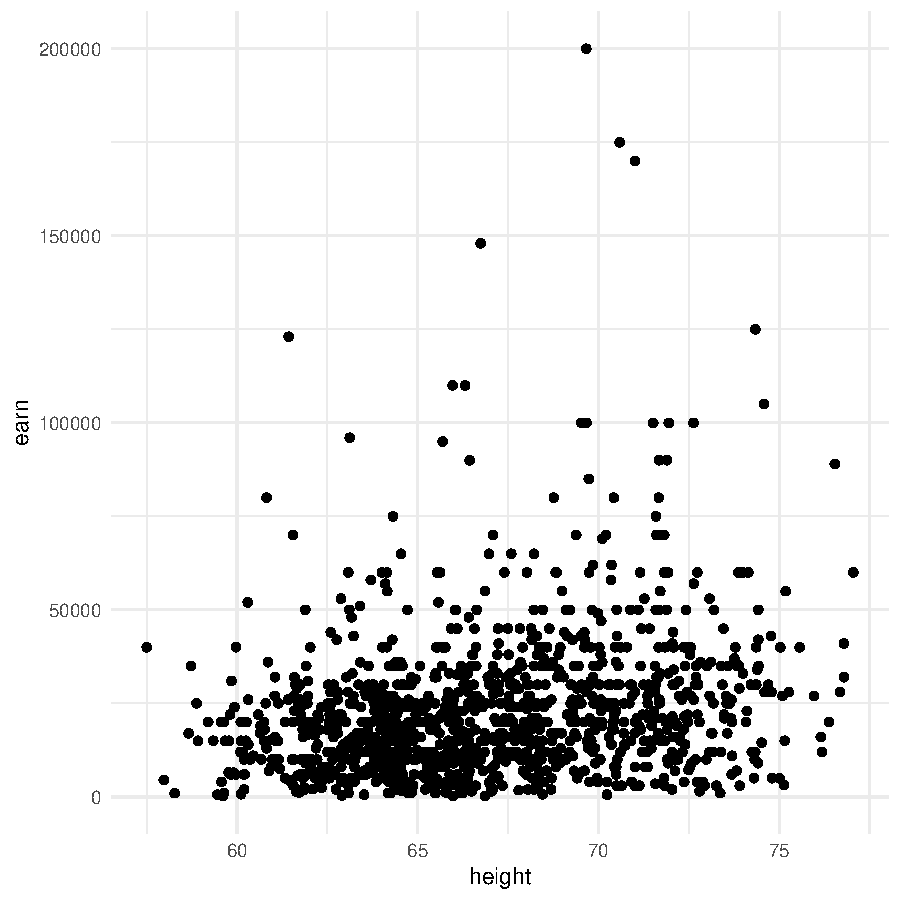
\includegraphics[width=.6\linewidth]{figure/assignment-03-ChattapadhyayKausik-Rnwauto-report-1} 

}


\begin{kframe}\begin{alltt}
\hlcom{## `age` vs. `earn`}
\hlkwd{ggplot}\hlstd{(heights_df,} \hlkwd{aes}\hlstd{(}\hlkwc{x}\hlstd{=age,} \hlkwc{y}\hlstd{=earn))} \hlopt{+} \hlkwd{geom_point}\hlstd{()}
\end{alltt}
\end{kframe}

{\centering 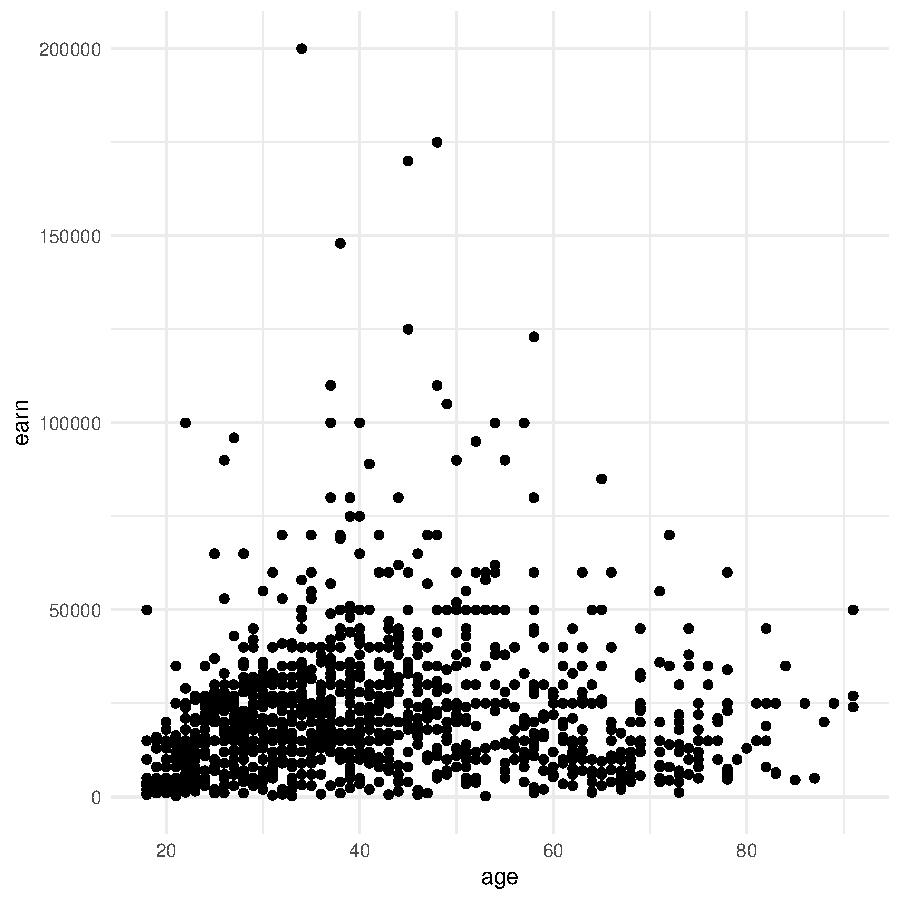
\includegraphics[width=.6\linewidth]{figure/assignment-03-ChattapadhyayKausik-Rnwauto-report-2} 

}


\begin{kframe}\begin{alltt}
\hlcom{## `ed` vs. `earn`}
\hlkwd{ggplot}\hlstd{(heights_df,} \hlkwd{aes}\hlstd{(}\hlkwc{x}\hlstd{=ed,} \hlkwc{y}\hlstd{=earn))} \hlopt{+} \hlkwd{geom_point}\hlstd{()}
\end{alltt}
\end{kframe}

{\centering 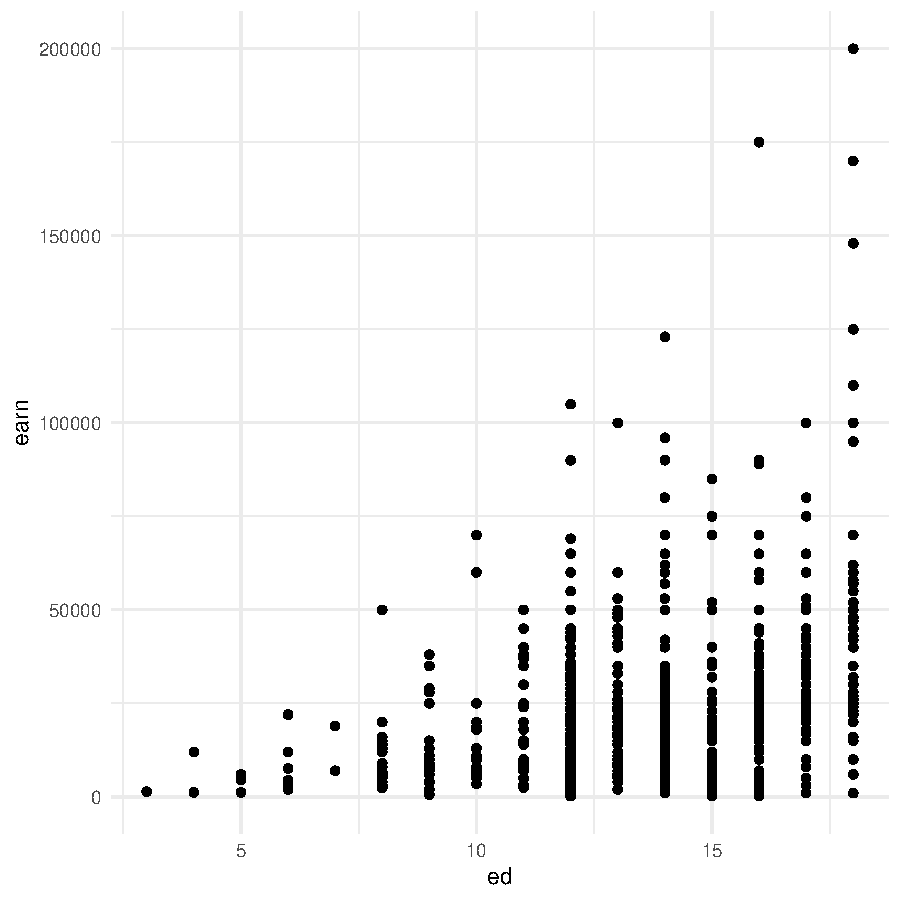
\includegraphics[width=.6\linewidth]{figure/assignment-03-ChattapadhyayKausik-Rnwauto-report-3} 

}


\begin{kframe}\begin{alltt}
\hlcom{## Re-create the three scatterplots and add a regression trend line using}
\hlcom{## the `geom_smooth()` function}
\hlcom{## `height` vs. `earn`}
\hlkwd{ggplot}\hlstd{(heights_df,} \hlkwd{aes}\hlstd{(}\hlkwc{x}\hlstd{=height,} \hlkwc{y}\hlstd{=earn))} \hlopt{+} \hlkwd{geom_point}\hlstd{()} \hlopt{+} \hlkwd{geom_smooth}\hlstd{()}
\end{alltt}


{\ttfamily\noindent\itshape\color{messagecolor}{\#\# `geom\_smooth()` using method = 'gam' and formula 'y \textasciitilde{} s(x, bs = "{}cs"{})'}}\end{kframe}

{\centering 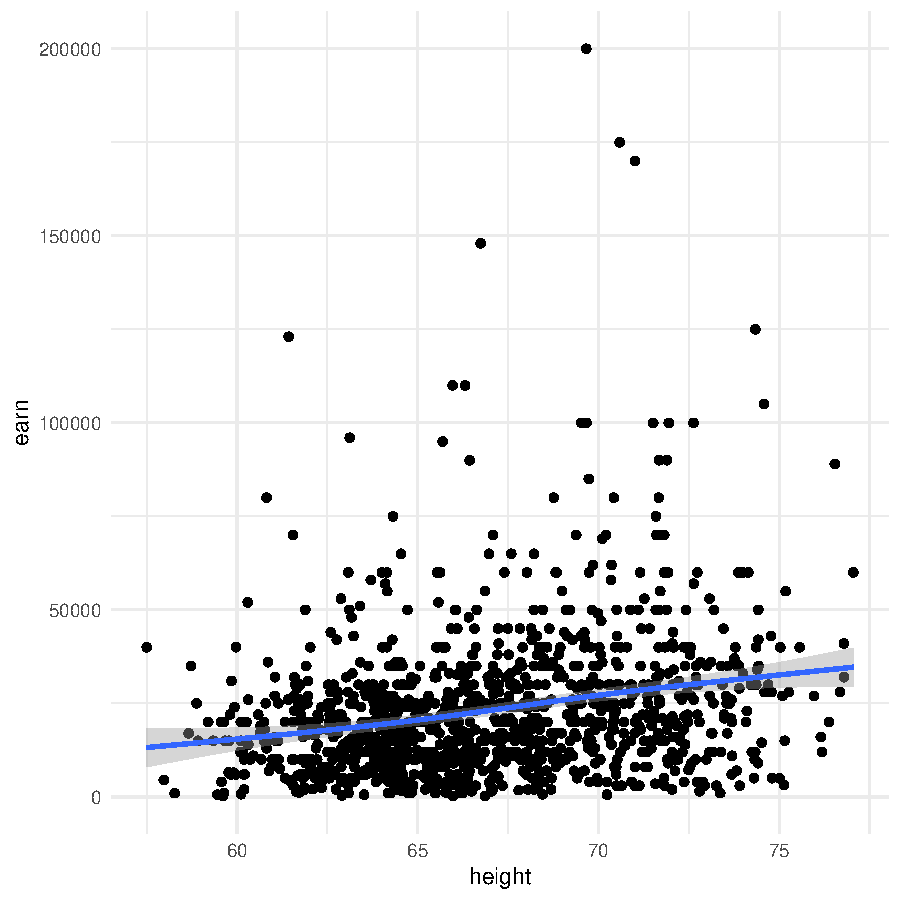
\includegraphics[width=.6\linewidth]{figure/assignment-03-ChattapadhyayKausik-Rnwauto-report-4} 

}


\begin{kframe}\begin{alltt}
\hlcom{## `age` vs. `earn`}
\hlkwd{ggplot}\hlstd{(heights_df,} \hlkwd{aes}\hlstd{(}\hlkwc{x}\hlstd{=age,} \hlkwc{y}\hlstd{=earn))} \hlopt{+} \hlkwd{geom_point}\hlstd{()} \hlopt{+} \hlkwd{geom_smooth}\hlstd{()}
\end{alltt}


{\ttfamily\noindent\itshape\color{messagecolor}{\#\# `geom\_smooth()` using method = 'gam' and formula 'y \textasciitilde{} s(x, bs = "{}cs"{})'}}\end{kframe}

{\centering 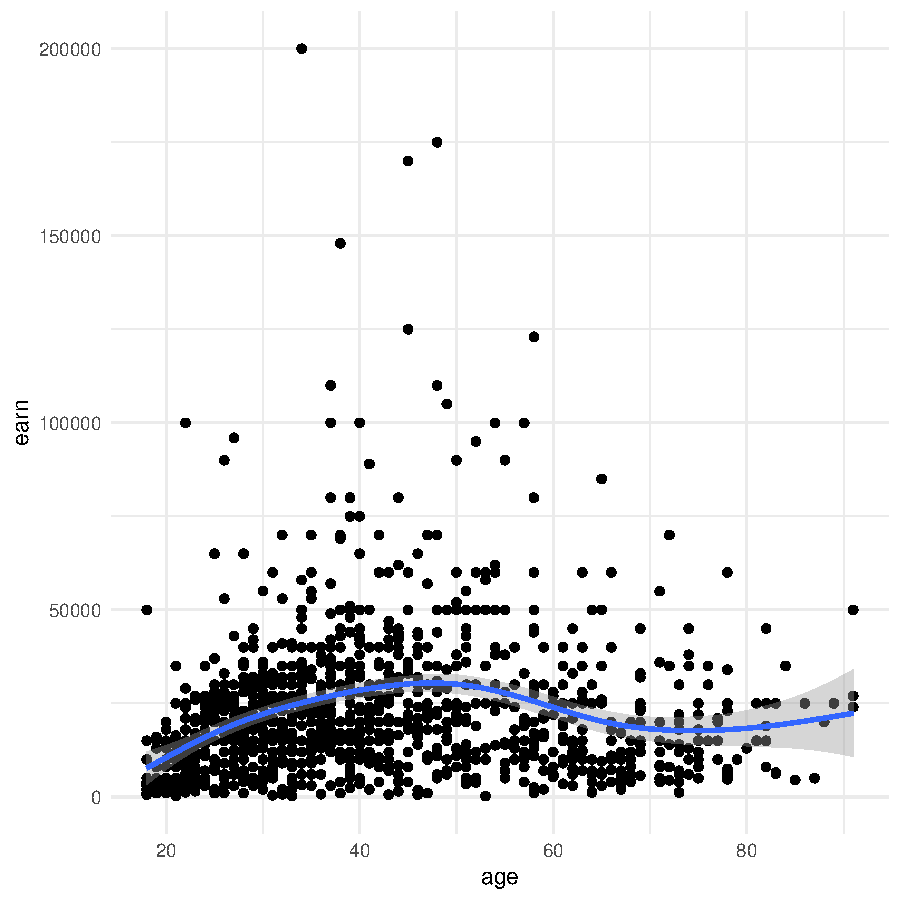
\includegraphics[width=.6\linewidth]{figure/assignment-03-ChattapadhyayKausik-Rnwauto-report-5} 

}


\begin{kframe}\begin{alltt}
\hlcom{## `ed` vs. `earn`}
\hlkwd{ggplot}\hlstd{(heights_df,} \hlkwd{aes}\hlstd{(}\hlkwc{x}\hlstd{=ed,} \hlkwc{y}\hlstd{=earn))} \hlopt{+} \hlkwd{geom_point}\hlstd{()} \hlopt{+} \hlkwd{geom_smooth}\hlstd{()}
\end{alltt}


{\ttfamily\noindent\itshape\color{messagecolor}{\#\# `geom\_smooth()` using method = 'gam' and formula 'y \textasciitilde{} s(x, bs = "{}cs"{})'}}\end{kframe}

{\centering 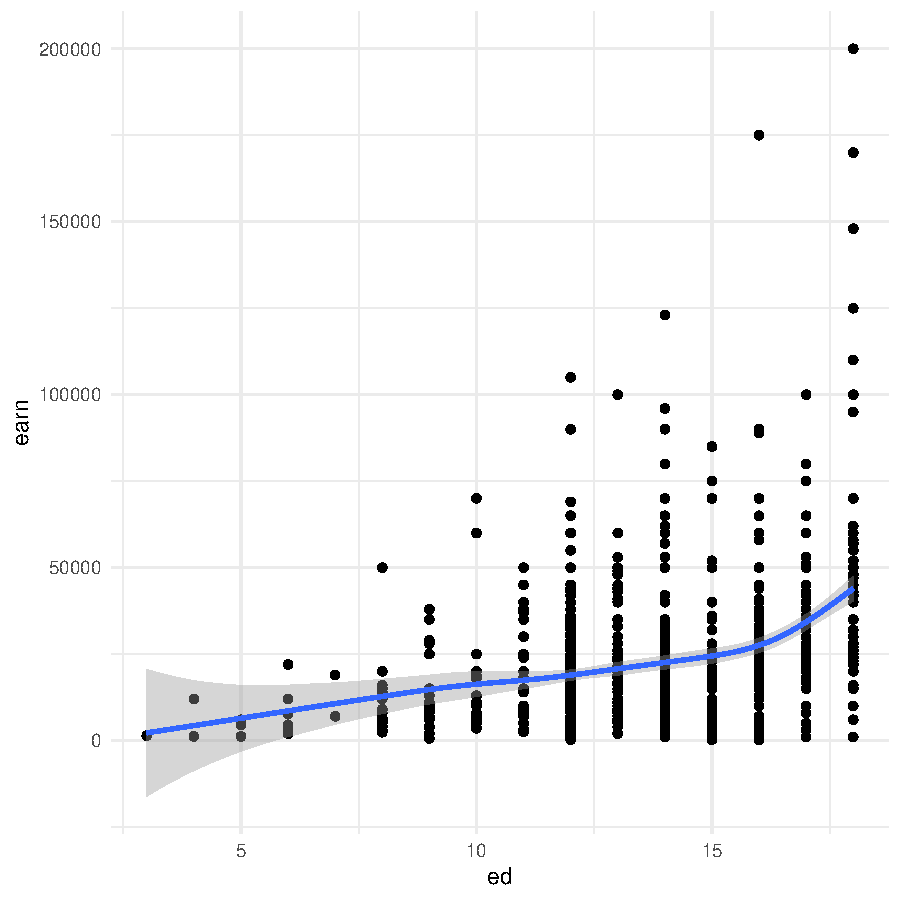
\includegraphics[width=.6\linewidth]{figure/assignment-03-ChattapadhyayKausik-Rnwauto-report-6} 

}


\begin{kframe}\begin{alltt}
\hlcom{## Create a scatterplot of `height`` vs. `earn`.  Use `sex` as the `col` (color) attribute}
\hlkwd{ggplot}\hlstd{(heights_df,} \hlkwd{aes}\hlstd{(}\hlkwc{x}\hlstd{=height,} \hlkwc{y}\hlstd{=earn,} \hlkwc{col}\hlstd{=sex))} \hlopt{+} \hlkwd{geom_point}\hlstd{()}
\end{alltt}
\end{kframe}

{\centering 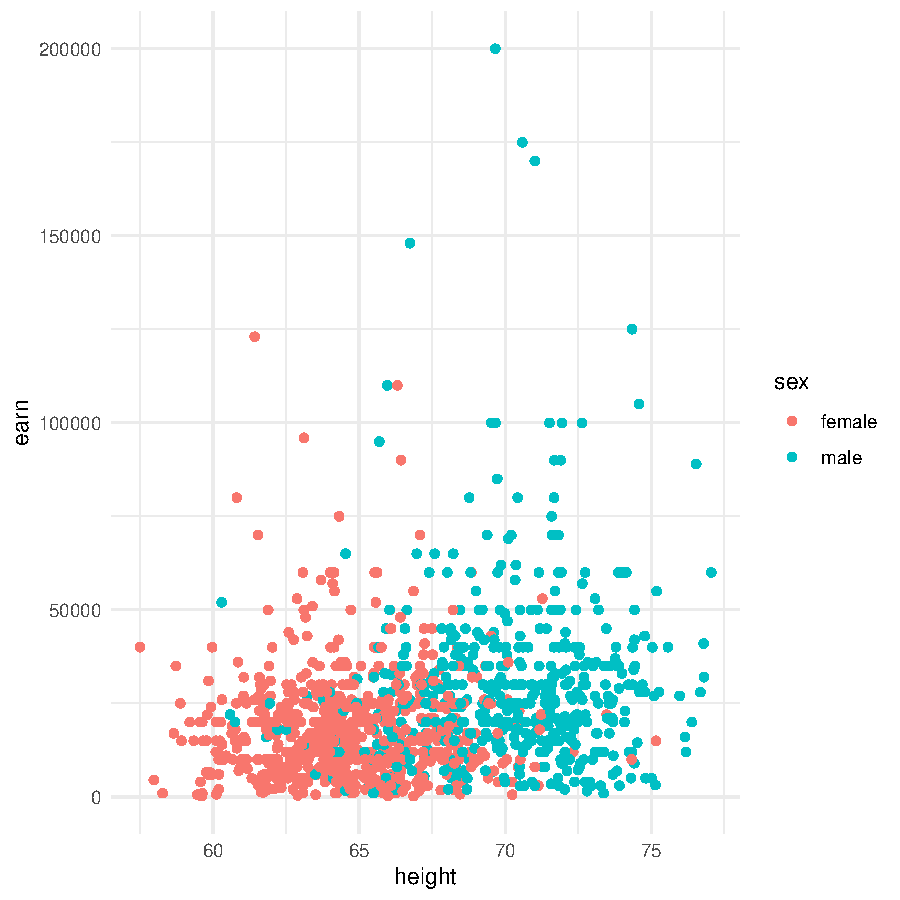
\includegraphics[width=.6\linewidth]{figure/assignment-03-ChattapadhyayKausik-Rnwauto-report-7} 

}


\begin{kframe}\begin{alltt}
\hlcom{## Using `ggtitle()`, `xlab()`, and `ylab()` to add a title, x label, and y label to the previous plot}
\hlcom{## Title: Height vs. Earnings}
\hlcom{## X label: Height (Inches)}
\hlcom{## Y Label: Earnings (Dollars)}
\hlkwd{ggplot}\hlstd{(heights_df,} \hlkwd{aes}\hlstd{(}\hlkwc{x}\hlstd{=height,} \hlkwc{y}\hlstd{=earn,} \hlkwc{col}\hlstd{=sex))} \hlopt{+} \hlkwd{geom_point}\hlstd{()} \hlopt{+}
        \hlkwd{ggtitle}\hlstd{(}\hlstr{"Height vs. Earnings"}\hlstd{)} \hlopt{+} \hlkwd{xlab}\hlstd{(}\hlstr{"Height (Inches)"}\hlstd{)}  \hlopt{+}
        \hlkwd{ylab}\hlstd{(}\hlstr{"Earnings (Dollars)"}\hlstd{)}
\end{alltt}
\end{kframe}

{\centering 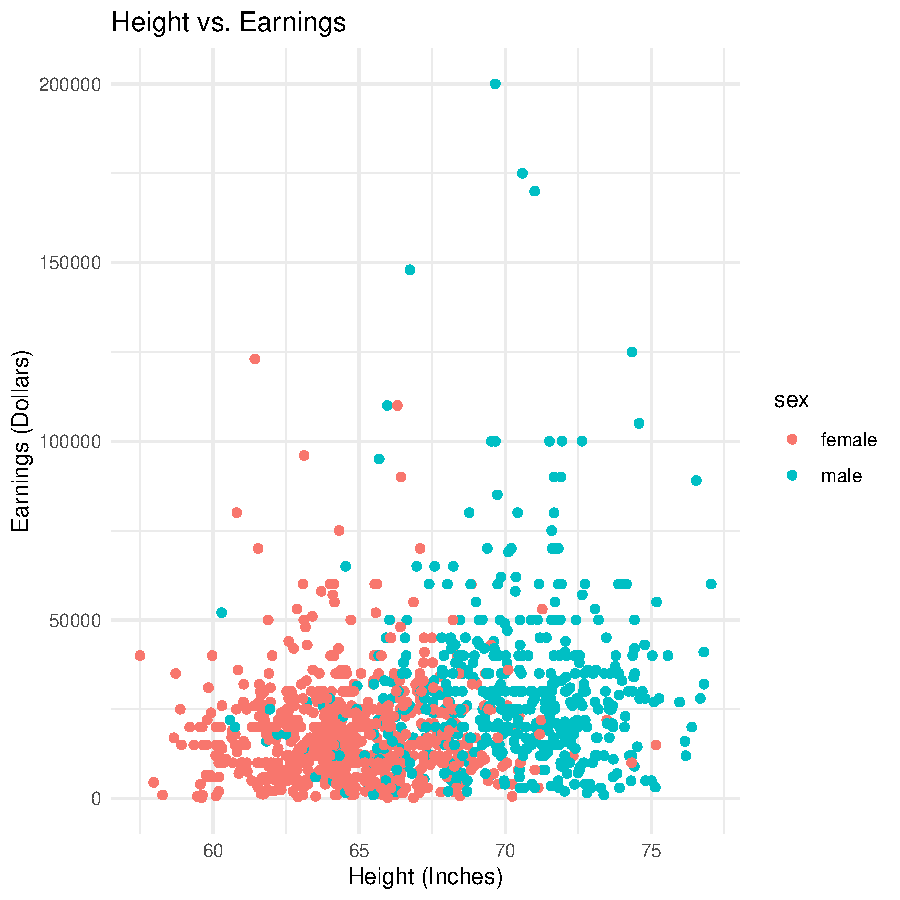
\includegraphics[width=.6\linewidth]{figure/assignment-03-ChattapadhyayKausik-Rnwauto-report-8} 

}


\begin{kframe}\begin{alltt}
\hlcom{# https://ggplot2.tidyverse.org/reference/geom_histogram.html}
\hlcom{## Create a histogram of the `earn` variable using `geom_histogram()`}
\hlkwd{ggplot}\hlstd{(heights_df,} \hlkwd{aes}\hlstd{(earn))} \hlopt{+} \hlkwd{geom_histogram}\hlstd{()}
\end{alltt}


{\ttfamily\noindent\itshape\color{messagecolor}{\#\# `stat\_bin()` using `bins = 30`. Pick better value with `binwidth`.}}\end{kframe}

{\centering 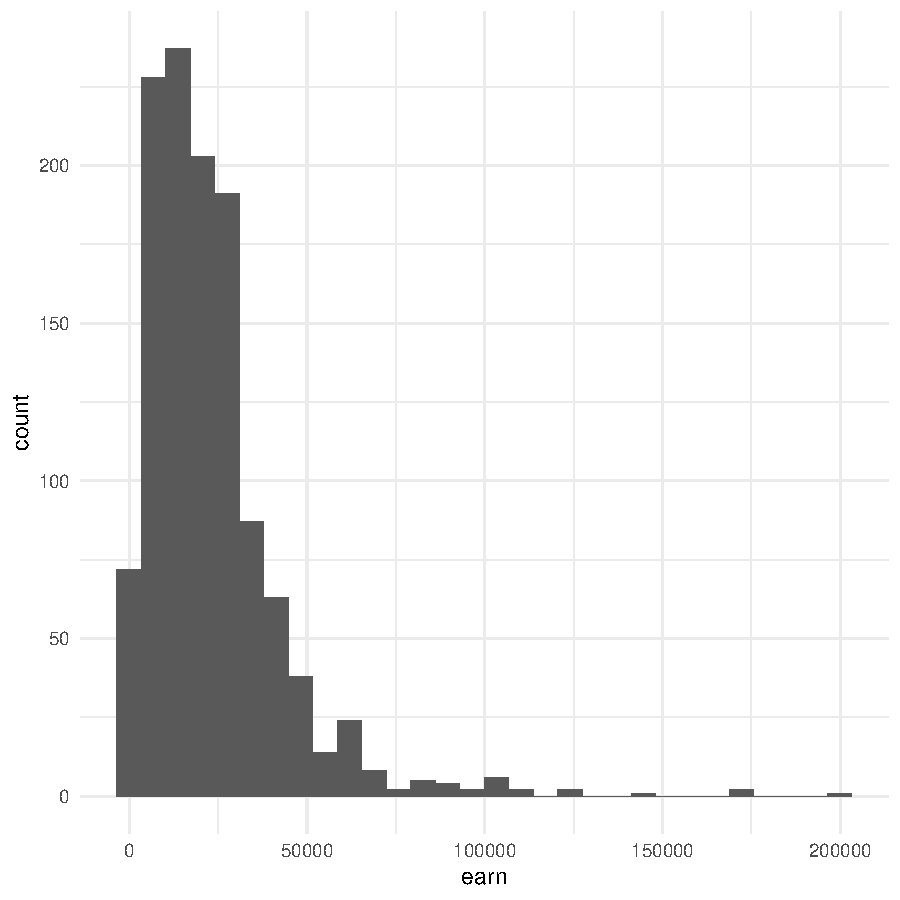
\includegraphics[width=.6\linewidth]{figure/assignment-03-ChattapadhyayKausik-Rnwauto-report-9} 

}


\begin{kframe}\begin{alltt}
\hlcom{## Create a histogram of the `earn` variable using `geom_histogram()`}
\hlcom{## Use 10 bins}
\hlkwd{ggplot}\hlstd{(heights_df,} \hlkwd{aes}\hlstd{(earn))} \hlopt{+} \hlkwd{geom_histogram}\hlstd{(}\hlkwc{bins} \hlstd{=} \hlnum{10}\hlstd{)}
\end{alltt}
\end{kframe}

{\centering 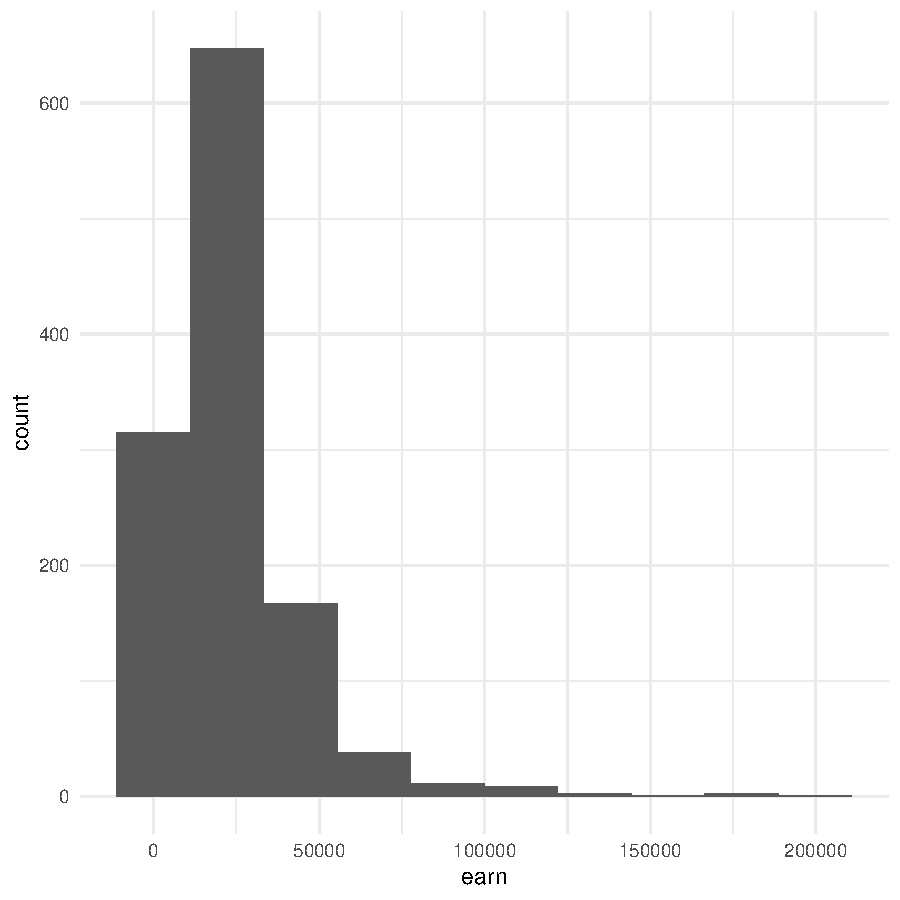
\includegraphics[width=.6\linewidth]{figure/assignment-03-ChattapadhyayKausik-Rnwauto-report-10} 

}


\begin{kframe}\begin{alltt}
\hlcom{# https://ggplot2.tidyverse.org/reference/geom_density.html}
\hlcom{## Create a kernel density plot of `earn` using `geom_density()`}
\hlkwd{ggplot}\hlstd{(heights_df,} \hlkwd{aes}\hlstd{(earn))} \hlopt{+}  \hlkwd{geom_density}\hlstd{(}\hlkwc{color}\hlstd{=}\hlstr{"darkblue"}\hlstd{,} \hlkwc{fill}\hlstd{=}\hlstr{"lightblue"}\hlstd{,} \hlkwc{linetype}\hlstd{=}\hlstr{"dashed"}\hlstd{)}
\end{alltt}
\end{kframe}

{\centering 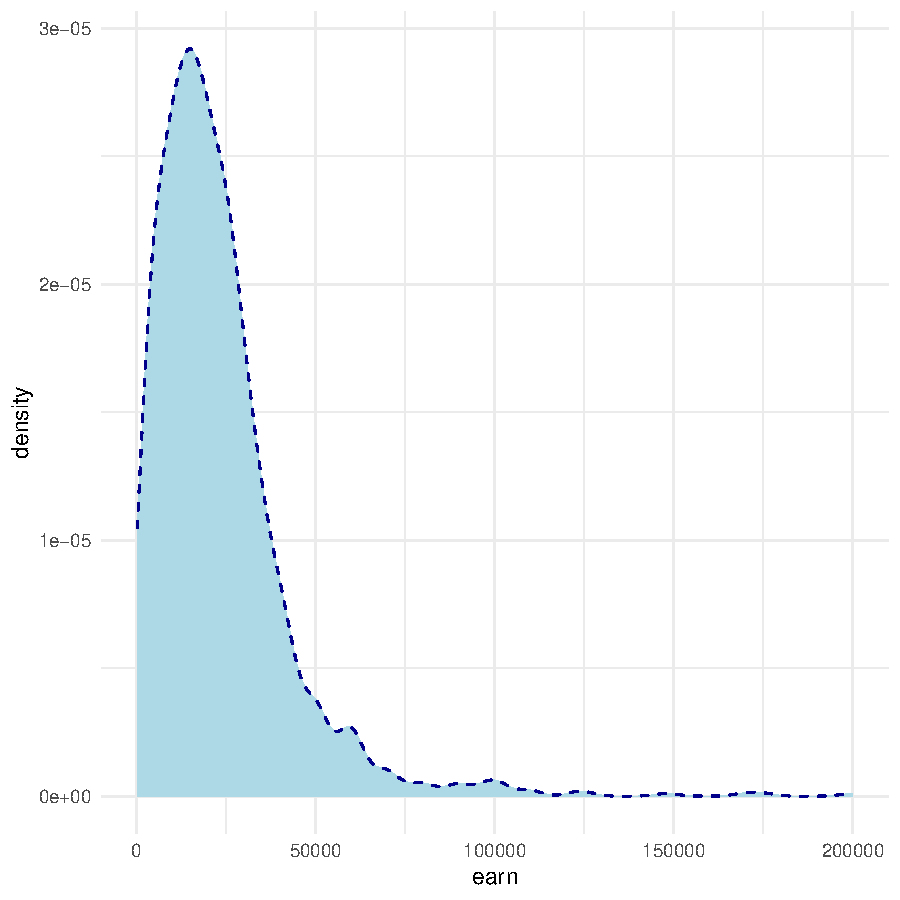
\includegraphics[width=.6\linewidth]{figure/assignment-03-ChattapadhyayKausik-Rnwauto-report-11} 

}


\end{knitrout}

The R session information (including the OS info, R version and all
packages used):

\begin{knitrout}
\definecolor{shadecolor}{rgb}{0.969, 0.969, 0.969}\color{fgcolor}\begin{kframe}
\begin{alltt}
\hlkwd{sessionInfo}\hlstd{()}
\end{alltt}
\begin{verbatim}
## R version 4.0.0 (2020-04-24)
## Platform: x86_64-apple-darwin17.0 (64-bit)
## Running under: macOS Catalina 10.15.7
## 
## Matrix products: default
## BLAS:   /System/Library/Frameworks/Accelerate.framework/Versions/A/Frameworks/vecLib.framework/Versions/A/libBLAS.dylib
## LAPACK: /Library/Frameworks/R.framework/Versions/4.0/Resources/lib/libRlapack.dylib
## 
## locale:
## [1] en_US.UTF-8/en_US.UTF-8/en_US.UTF-8/C/en_US.UTF-8/en_US.UTF-8
## 
## attached base packages:
## [1] stats     graphics  grDevices utils     datasets  methods   base     
## 
## other attached packages:
## [1] ggthemes_4.2.4  scales_1.2.1    lubridate_1.8.0 ggplot2_3.3.6   rjson_0.2.21   
## [6] jsonlite_1.8.0  DBI_1.1.3       readxl_1.4.0   
## 
## loaded via a namespace (and not attached):
##  [1] Rcpp_1.0.8.3      cellranger_1.1.0  pillar_1.8.1      compiler_4.0.0   
##  [5] highr_0.9         tools_4.0.0       digest_0.6.29     bit_4.0.4        
##  [9] lattice_0.20-45   nlme_3.1-147      viridisLite_0.4.1 RSQLite_2.2.12   
## [13] memoise_2.0.1     evaluate_0.16     lifecycle_1.0.1   tibble_3.1.6     
## [17] gtable_0.3.1      mgcv_1.8-40       pkgconfig_2.0.3   rlang_1.0.2      
## [21] Matrix_1.4-1      cli_3.2.0         rstudioapi_0.14   xfun_0.30        
## [25] fastmap_1.1.0     withr_2.5.0       stringr_1.4.1     knitr_1.40       
## [29] generics_0.1.3    vctrs_0.4.0       bit64_4.0.5       grid_4.0.0       
## [33] glue_1.6.2        R6_2.5.1          fansi_1.0.3       purrr_0.3.4      
## [37] farver_2.1.0      blob_1.2.3        magrittr_2.0.3    splines_4.0.0    
## [41] ellipsis_0.3.2    colorspace_2.0-3  labeling_0.4.2    utf8_1.2.2       
## [45] tinytex_0.41      stringi_1.7.6     munsell_0.5.0     cachem_1.0.6     
## [49] crayon_1.5.1
\end{verbatim}
\begin{alltt}
\hlkwd{Sys.time}\hlstd{()}
\end{alltt}
\begin{verbatim}
## [1] "2022-09-11 16:10:43 EDT"
\end{verbatim}
\end{kframe}
\end{knitrout}


\end{document}
